% !TEX TS-program = pdflatex
% !TEX encoding = UTF-8 Unicode

% This is a simple template for a LaTeX document using the "article" class.
% See "book", "report", "letter" for other types of document.

\documentclass[10pt, conference, compsocconf, letterpaper]{IEEEtran} % use larger type; default would be 10pt

\usepackage[utf8]{inputenc} % set input encoding (not needed with XeLaTeX)

%%% Examples of Article customizations
% These packages are optional, depending whether you want the features they provide.
% See the LaTeX Companion or other references for full information.

%%% PAGE DIMENSIONS
%\usepackage{geometry} % to change the page dimensions
%\geometry{a4paper} % or letterpaper (US) or a5paper or....
% \geometry{margins=2in} % for example, change the margins to 2 inches all round
% \geometry{landscape} % set up the page for landscape
%   read geometry.pdf for detailed page layout information

\usepackage{graphicx} % support the \includegraphics command and options

% \usepackage[parfill]{parskip} % Activate to begin paragraphs with an empty line rather than an indent

%%% PACKAGES
\usepackage{booktabs} % for much better looking tables
\usepackage{array} % for better arrays (eg matrices) in maths
\usepackage{paralist} % very flexible & customisable lists (eg. enumerate/itemize, etc.)
\usepackage{verbatim} % adds environment for commenting out blocks of text & for better verbatim
\usepackage{subfig} % make it possible to include more than one captioned figure/table in a single float
% These packages are all incorporated in the memoir class to one degree or another...
\usepackage{algorithm}
\usepackage{algpseudocode}
\usepackage{amsthm}
\usepackage[font=small,labelfont=bf]{caption}


%%% HEADERS & FOOTERS
\usepackage{fancyhdr} % This should be set AFTER setting up the page geometry
\pagestyle{fancy} % options: empty , plain , fancy
\renewcommand{\headrulewidth}{0pt} % customise the layout...
\lhead{}\chead{}\rhead{}
\lfoot{}\cfoot{\thepage}\rfoot{}

%%% SECTION TITLE APPEARANCE
%\usepackage{sectsty}
%\allsectionsfont{\sffamily\mdseries\upshape} % (See the fntguide.pdf for font help)
% (This matches ConTeXt defaults)

%%% ToC (table of contents) APPEARANCE
%\usepackage[nottoc,notlof,notlot]{tocbibind} % Put the bibliography in the ToC
%\usepackage[titles,subfigure]{tocloft} % Alter the style of the Table of Contents
%\renewcommand{\cftsecfont}{\rmfamily\mdseries\upshape}
%\renewcommand{\cftsecpagefont}{\rmfamily\mdseries\upshape} % No bold!

%%% END Article customizations

%%% The "real" document content comes below...

\title{Reducing Traffic and Delays in P2P Systems with Replicated Mutable Files}
\author{
Andrew Rosen \qquad Brendan Benshoof \qquad Matt Johnson \qquad Anu Bourgeois  \\Department of Computer Science, Georgia State University\\ 34 Peachtree St NW \\ Atlanta, Georgia 30303\\  rosen@cs.gsu.edu }
%\date{} % Activate to display a given date or no date (if empty),
         % otherwise the current date is printed 

\begin{document}
\maketitle

\begin{abstract}
Peer-to-peer networks generate an increasing amount of traffic each year as they become more widely used and as larger files become more common to share. This has led research into how peer-to-peer networks can be used for tasks such as keeping mutable files across a network up-to-date and using other points in the network to store temporary copies of the file to ease the load on the server by diverting traffic. The integrated file replication and consistency maintenance algorithm (IRM) combined the problems into one and examined the effects on a network using Chord. This paper proposes reducing the strain on the file owners by reducing polling and diverting  polling traffic to the replica nodes.  These changes can be accomplished without decreasing the hit rate at the replica nodes, while also decreasing the overall traffic in the network and average latency.
\end{abstract}



\section{Introduction}
Peer-to-peer (P2P) networks are of enormous interest to network research, as they provide an efficient way to distribute large files to millions of users without many of the limitations of the traditional client-server model. In the client-server model, the server addresses each client's request individually, creating a single point of failure due to traffic or the loss of the server.  In peer-to-peer networks, each node takes on both the role of client and server.  If someone wishes to introduce data into the a peer-to-peer network, peers can both request the file and distribute it to others.  This takes much of the burden of file distribution off of what would have normally been an extremely busy server \cite{Overview}.

P2P networks have resulted in an unprecedented amount of data being purveyed through the Internet.  While recent studies show that P2P accounts for 13.2\% of downstream traffic, down from its peak of 40\% of all Internet traffic, the actual volume of P2P traffic is at its highest yet \cite{5713296}. Many companies have embraced legal uses of P2P technology, such as providing ways to stream media or provide large updates  \cite{P2PLegal}.  For example, Blizzard uses a modified BitTorrent protocol to distribute updates and patches to millions of users for games such as World of Warcraft and Starcraft II \cite{chehai2006analysis}.

Because files in P2P networks create connections that last for an extended period of time and handle files that can have quite large sizes, reducing the overhead of these networks is utterly crucial in making them efficient. One common method of reducing network traffic is file replication \cite{IRM}, in which strategically placed peers create local copies of popular files\footnote{It is important to note that the peer creating a replica might have no use for the file; it is creating the replica to help the network.}.  These replicas are then able to respond to file requests, diverting traffic away from the file owner.  However, as applications implementing P2P to distribute data between users become more elaborate, new complications are introduced, such as distributing a file that changes over time.  

If a mutable file is being shared across the network, the file replication process becomes profoundly more complex as the replicas  now need to make sure their contents are up-to-date \cite{IRM} by communicating with the server.  This paper examines a modification of IRM, short for \textit{integrated file replication and consistency maintenance}, an algorithm proposed in \cite{IRM}. This protocol views the tasks of intelligently placing replicas and keeping files up-to-date to be intertwined.  After all, the objective of creating a replica is to \emph{reduce} the load on the server or file owner, whereas the task of keeping a mutable file up-to-date requires constant polling of the file owner, \emph{increasing} the number of messages inbound.     

We propose that by letting the nodes delay polling, while allowing them to take on additional responsibilities, will reduce the network traffic and burden placed on the file owners.

Section II provides background information.  Section III discusses the previous work this paper is based on.  Section IV presents our modifications.  Section V discusses the specifics of our simulation setup and the various parameters.  Section VI examines the results of the simulations.  Section VII concludes the paper with avenues for future research.  All code required for the simulation is being released under the MIT license and can be acquired via github \cite{IRMLP}.  





\section{Background}
Not all peer-to-peer networks are equal; there are variety of protocols and methodologies that a networks could implement and this affects what kind of solutions are available to reduce the traffic on the network    \cite{SurveyCompare} \cite{Overview}.
%\subsection{Basic Peer-to-Peer Networks}
The most basic type of network is a structured, centralized  network.  Peers in this network communicate with a central server to provide their files and to locate other peers that have the files they are searching for.  This is structured in the sense that the layout of the overlay network is tightly controlled, in this case by the server(s). While this avoids the problems of routing, it has the same issues of scalability as a client-server layout and is not much of an improvement. An example of this network is the long defunct Napster  \cite{SurveyCompare} \cite{Overview}.

On the other side of the spectrum, there are unstructured, decentralized networks.  These networks create overlay links between nodes in a random manner. This leads to a very unstructured overlay, but it is one that is very easily constructed.  No single node is responsible for the whole of the network;  files are located by sending out requests to neighboring peers, which in turn request from their neighbors and so on. Should a file become suddenly popular, this flood of this requests can easily bring some peers to their knees, unable to deal with the high level of traffic \cite{Lv:2002:SRU:514191.514206}.  This makes these types of networks also a poor choice for implementation \cite{Overview}.

%\subsection{DHT-based Peer-to-Peer Networks}
Modern P2P implementations are hard to classify easily, due to the variety of methods used to create a working network that avoids the weaknesses of the two above network types.  Many networks today use a decentralized structured approach to distribute files, where the topology of the overlay is constructed and controlled by the protocol and the information about the network is distributed among the peers.  This distribution is typically accomplished by a distributed hash table (DHT).  Networks that use a DHT choose specific peers in which to place information about how to find particular files or data.  These peers are chosen so that the peer's ID in the network corresponds to the file or data's ID, typically by hashing both ID's and comparing them  \cite{SurveyCompare}. 

In addition, the network topology is distributed among various peers.  Each peer has a table consisting of other peers in the network and the means of communicating with them.  The contents of this table are also controlled by the protocol.  The table handles the routing of requests from one node to another; when a peer receives a request it cannot fulfill, such as information about where to find a particular file, it directs the the request to the node that is "closest" to the destination of the request. How this works is determined by each protocol \cite{Chord}.  It should be noted that closeness is relative to the algorithm; depending on what identifiers are assigned, a node in New York City might be "close" to a node in Russia, but "far" from a node physically located only miles away.  Examples of protocols that use these techniques are trackerless BitTorrent \cite{BitTorrent}, Chord \cite{Chord}, and Kademlia \cite{Kademlia}. As our work is implemented using Chord, we provide more detail here. 

Chord uses hashing and mapping functions to efficiently disseminate information throughout a network, using keys and nodes.  Keys can be identifiers for data, such as keywords and tags; the associated data would be the values under this mapping.  Chord takes peers in the network and gives them a node ID.  Both the keys and the nodes are hashed to produce an identifier of length $m$, $m$ being some value large enough that the hashing function would be extremely unlikely to assign two different nodes or keys the same hashed identifier.  For the sake of clarity, both the node ID and key refers to the corresponding hashed value in the following description.

Chord takes the nodes and structures them into a circle composed of less than $2^m$ nodes, ordered clockwise by identifier from lowest to highest.  Chord then takes the keys and places each in the node that has the same hashed identifier as it or the node with the first identifier that follows this value.  The node that takes some key $\kappa$ is known as the $successor$ of $\kappa$, or $successor(\kappa)$.  

Since this is a circle of maximum size $2^m$, the assessment is done in modulo $2^m$.  Given $K$ keys and $N$ nodes, each node will end up being responsible for approximately \(K\over N\) keys.

Each node could then find  the information of a key by asking the next node in the circle for the information, who would then pass the request through the circle until the node with the identifier equal or first succeeding the value of the key was found.  That node would be then be able to pass the data, should it exist, back to the requesting node.  This naive approach is largely inefficient, but provides a base example on how nodes in Chord search for information.

To aid in searching, each node stores the locations of up to $m$ other nodes in the network.  Specifically, entry $i$ in the "finger table" of a node with the id of $n$ will be the location of $successor(n+2^{i-1})$ $mod$ $2^m$. When a node wants to find some key, it looks to the entry in the finger table that will get it closest to the key without going past and request that information in the manner described above.  Fig ~\ref{net} \cite{Chordpic} gives an example network with a node pointing to the other nodes it knows the location of. This approach allows nodes to find a specific key in $O(log_mn)$ time.  For a more detailed explanation and psuedocode, please refer to Stoica \emph{et al.}'s paper on the Chord protocol \cite{Chord}.

\begin{figure}
\includegraphics[width=\linewidth]{Chordnetwork}
\caption{In this 16 node network, $m=4$.}
\label{net}
\end{figure}




\section{Integrated File Replication and Consistency Maintenance}

%Issues with P2P networks and static files is an area that is well defined

The interaction of P2P networks and stale files in a well defined area of research.   However, the addition of a file or files that are rapidly updated changes the way many aspects of a peer-to-peer network works.  One approach to handle this change is to replicate files across the network.

File replication is often used as a strategy to reduce the load on a server due from hosting a popular file or sudden spikes in demand.  The exact methodology depends on the type of P2P network, but the basic idea is the same: the network assigns certain peers that are forwarding a large amount of file requests to hold a replica of that file.  However, if the file in question is one that changes periodically, then the network must have some mechanism to maintain up-to-date copies of the files on all the nodes acting as replicas.  Depending on how these replicas are chosen and how the replicas keep up-to-date, the overhead for file consistency can be quite costly.

H. Shen presents a method called IRM \cite{IRM} in which individual nodes, rather than the owner(in this case, the server being the owner of the file being updated) make autonomous decisions about becoming replicas.   IRM significantly reduces the amount of overhead caused from update messages and removes unnecessary replicas from the network by combining the two processes of replica creation and consistency maintenance. The basic scheme is briefly discussed below.


\subsection{Replica Creation}
The goal of creating replicas is to reduce the load on the original owner of the file.  Requiring the file owner to identify where replicas should be placed would require massive amounts of data about the topology and is computationally expensive.  Since we are aiming to decrease the burden on the file owners, we need to instead hand give this responsibility to each individual node.  Each node should elect to become a replica without collaboration with other nodes.


Under IRM, a node uses two different criteria to determine whether or not it should replicate some file: how often the node requests that file and how often the node forwards requests for that file. Once the rate a which a node makes or forwards requests exceeds either predefined threshold, it creates a replica of that file. 

The node stores a copy of each file it becomes a replica for and responds to requests for the file as though it were the original owner.  If a node neither forwards nor requests a file often enough, that replica is deleted\footnote{There is nothing stopping a node from becoming a replica again once the request/forward rates pick back up.}.


Ideally, this process will create replicas that takes the pressure off of nodes experiencing a sudden spike in traffic.  If the original file never changes, then the replica can store the file and reply to requests without having to check in with the owner.  However, if the file is one that changes over time, additional work is needed to make sure that the replica is up-to-date.


\subsection{Consistency Maintenance}
Once a replica  is created, it will need to periodically poll the file's owner for changes.  Poll too little and the replica risks giving other nodes stale data; if nodes poll too often, the combined polling of multiple replicas will overwhelm the file owner and possibly the entire network.  While it is impossible for replicas to guarantee that they will always provide the latest copy of the data \cite{Gilbert:2002:BCF:564585.564601}, we can create polling schemes to ensure that there is a very low incidence of stale files. 

IRM uses an adaptive polling algorithm to poll more often when the original file is likely to have changed and to reduce polling during periods where the file unlikely to have changed.  This is done by adjusting the interval at which a file is polled, called the \textit{time-to-refresh} ($TTR$), based on the polling responses for that file.  If a poll reveals that the file is unchanged, we can wait slightly longer to poll.  However, if the file has changed, we decrease the $TTR$ to poll more often.   The increase rate is additive, while the decrease rate is multiplicative, letting the node "home in" on the actual rate of change for the file. 

$TTR$ is bound by both a minimum and a maximum; the polls will never occur quicker than a file can update, but the polls will not be so slow. In addition, the polling will also never exceed the rate at which the replica answers request for data.  For example, say that a replica's $TTR$ was 5 seconds, but it receives a request for data every 15 seconds (on average).  There would be 2 wasted polling operations as the replica would needlessly update its data twice before it responded to a request.

Not discussed in the original paper but worth mentioning is that by being adaptive to polling in this manner also accounts for the latency of sending messages.




\subsection{Original Simulation Results}
When implemented on Chord, IRM performed exceeding well as compared to other algorithms, creating fewer replicas on average which were guaranteed by the algorithm to be highly utilized.  Furthermore, simulation results showed that the effectiveness of IRM at reducing hot-spots far surpassed the other algorithms tested.  IRM also produces much less traffic from its polling, as the polling rates are adaptive.  Finally, the simulation environment showed that the replicas produced a very low number of stale files -  below the 1\% range.

%However, the simulations were performed on networks where a great many number of files were immutable.   The network size was also not varied  CONTINUE DESCRIBING

%\subsection{IRM With Conditional}

%The simulation results showed consistantly exceptional results for IRM.  Our goal with Conditional is to further lighten the load on the network with a minimal hit to accuracy, if at all.

%Conditional functions as a modified version of IRM and, as such, works in much the same way.  First, Conditional creates replicas in the same manner as IRM, using the same parameters for query and forwarding thresholds.  However, rather than polling at some TTR, we poll whenever we initiate a query or when we forward a message iff dictated by TTR.  It can be easily seen that we have would experience fewer polls.





\section{Proposed Work}

Our proposed algorithm focused on four different modifications.  Together, they act to reduce polling, route further stress away from file owners, and decrease the amount of stale data given to file requesters.
 
Improving the polling rate without severely reducing the hit rate can only be done by reducing the number of polling messages that are wasted.  As demonstrated in the example from the previous section, a poll message (and its corresponding response) is wasted if the replica changes before it is accessed.  However, naively reducing the number of polls serves only to make the incidence of stale data more common.


Improving the hit rate is accomplished by reducing the size of a the window where a replica responds with stale data.  This can happen when the file has changed while the replica has yet to poll, the file changes while a poll response is in transit, or the data changing en route to the requester.

Routing stress away from file owners can be done indirectly by lowering the number of polling messages, or directly by letting replicas take on some more of the owner's responsibilities, such as responding to polls.

We now propose our four modifications.



\subsection{Greedy Polling}
If the polls are traveling along the DHT layer, then chances are that the nodes will be forwarding a number of polling responses for files they have replicated themselves.  By examining the polls it is forwarding, it can update both the replica and its $TTR$  without actually polling itself. We call this \emph{greedy polling}.

Whenever a node gets a poll response destined  for another replica, it checks to see if the poll response was for a file the node has a replica of as well.  If the poll response indicates that this node's replica is stale, it cuts its $TTR$ rate to poll sooner and updates the replica\footnote{Assuming that the data and poll response is bundled together, which was the case for our simulations.}.  If the replica is not out of date, no action is taken.  A description of this process is given by Algorithm. \ref{greedy}.


\begin{algorithm}                      % enter the algorithm environment
\caption{Greedy Polling}          % give the algorithm a caption
\label{greedy}                           % and a label for \ref{} commands later in the document
\begin{algorithmic}[1]                    % enter the algorithmic environment
	\State The node receives a poll response to forward
	\If{the response is for a file the node replicated}
		\If{The replica is up-to-date}
			\State $TTR \Leftarrow TTR + \alpha$
		\Else \Comment The replica is stale
			\State Update the replica
			\State $TTR \Leftarrow TTR \div \beta$
		\EndIf
		\If{$TTR > TTR_{max} $ or $TTR < TTR_{min} $ }
		\State Set $TTR$ back in bounds.
	\EndIf
	\If{$TTR < rate_{query}$}
		\State $TTR \Leftarrow rate_{query}$  
	\EndIf
		\State Calculate the next time to poll
	\EndIf
	\State Forward the poll response.
\end{algorithmic}
\end{algorithm}




\subsection{Lazy Polling}
We can further eliminate unnecessary polling by delaying when we initiate them.  Since our data needs to only be up-to-date when we have to handle file requests, we can delay checking if our file is up-to-date until then. Under Lazy Polling, we only check if we need to poll when we query or receive a file request.  Once that is done, we increase our $TTR$ by $\alpha$ if the data is current, or divide by $\beta$ if our data was stale.  

Essentially, rather than performing the IRM process every time interval, we wait until the last moment to do it. This modification synergizes extremely well with the greedy polling and poll interception processes.  The process is formally described by Algorithm~\ref{lazy}. 




\begin{algorithm}                      % enter the algorithm environment
\caption{Lazy Polling, based off IRM \cite{IRM}}          % give the algorithm a caption
\label{lazy}                           % and a label for \ref{} commands later in the document
\begin{algorithmic}[1]                    % enter the algorithmic environment
\State The replica receives a file request
\If{$TTR$ indicates the replica may be stale}
	\State Send out a poll
	\State Handle file request \Comment See subsection $D$
	\State Get poll response
	
	\If{Replica is still valid}
		\State $TTR \Leftarrow TTR + \alpha$
	\Else \Comment The file is stale.
		\State $TTR \Leftarrow TTR \div \beta$
	\EndIf
	\If{$TTR > TTR_{max} $ or $TTR < TTR_{min} $ }
		\State Set $TTR$ back in bounds.
	\EndIf
	\If{$TTR < rate_{query}$}
		\State $TTR \Leftarrow rate_{query}$  
	\EndIf
	
	\State Calculate next time to poll
\Else
	\State Respond to the data request with the replica
\EndIf

\end{algorithmic}
\end{algorithm}



\subsection{Poll Interception}
The primary reason nodes do not poll the file owners as frequently as possible is the risk of overwhelming both the file owner and the network.  By allowing replicas to take over some of that work, we can reduce that load even more.

 So long as a node's replica is more up-to-date than some other node's replica, it can respond to polls as though it were the file owner.  A replica that can be trusted to give other nodes in the network up-to-date copies of a file can be trusted to give an accurate poll response, so the impact on the hit-rate is minimal, if any\footnote{Assuming of course, the two nodes are not polling each other, which cannot happen under Chord.}.  This process will take the additional load off the file owners by decreasing the number of polls they receive.  In addition we can prove that by handling polling messages, we can decrease the overall network traffic.
 

\newtheorem*{Theorem}{Theorem}

\begin{Theorem}
Intercepting messages reduces average latency over time
\end{Theorem}

\begin{proof}
Consider two nodes on a Chord network, where node $a$ is the file requester and node $b$ is the file owner.  

Like any other arbitrary pair of node in a Chord network, the average distance is approximately equal to the distance separating any other arbitrary pair ($O\log n$).  Let $r =$ this average distance.

Thus, a naive round trip time ($RTT$) on a Chord network without IRM nor IRM/LP, is 
$$RTT \approx 2r$$

Let us consider the case of a poll request for a file owned by $b$ being sent by a replica node $q$ on the path from $a$ to $b$, and received by a second replica node $p$.  We can find two distances: $$\delta_0 = distance(a, q)$$ and $$\delta_1 = distance(p,b)$$   

Assuming  $p$ and $q$ exist and $p$ is distinct from $b$, the minimum value for $\delta_0$ is 0 because $a$ could be a query based replica and $\delta_1$ is 1, because $p$ is distinct from $b$.  This gives a new value $RTT_0$ that occurs only when polls are intercepted.

$$RTT = 2r - \delta_0 -\delta_1$$


However, this new value is a worst-case of a poll interception that will arise only a fraction of the time.  If we look at the behavior over time, we can  calculate an upper bound for the average round-trip time of any message originate from $a$ and sent to $b$

$$RRT_{upper}= 2r - P(q)\times0 - P(p)\times1$$ 

Where $P(q)$ represents the probability that $q$ exists, corresponding to our recorded poll interception rate, and $P(p)$ represents the probability $p$ exists, corresponding to the percentage of file requests handled by replicas. Since the worst case is that $a$ is a query based replica we lose the benefit of $\delta_0$ in this evaluation, leaving use with

$$RRT_{upper}= 2r - P(p) \leq RTT $$

This means that the average $RTT$ of the network is lower for every poll intercepted and message handled by a replica. We could decrease the provable bound on $RTT$ by removing query based replicas, but this is not suggested because while lowering upper bound we have hurt the rate at which replicas handle file requests.
\end{proof}

%won't reduce path  as chord is circular, so routes are all different to and from


\subsection{Handling Request During Outstanding Polls}
When a replica receives a request for a file while it is in the middle of making a poll, it has some options for handling that request, summarized in Table~\ref{choice}.  

The simplest option is to respond to the request for data normally with the data on hand.  This option is easy to implement, guarantees a quick response, and keeps with the idea that the replica should take weight off the file owner.  However, this option sends data that has a much higher chance of being stale.

A more practical option is to wait for the poll to return, which is effectively what IRM proposes.  The benefit of this is that the node will not respond with a stale file\footnote{Assuming data does not change between the poll response and the requester receiving the data.}.  However, this means the node has to wait to take action until the poll returns, which could be a considerable amount of time if the file owner is overwhelmed or down, and requires additional space to store the messages until the poll returns.


The third option is to forward the message upstream, as though the node being polled did not have a replica of the data. This option avoids increasing the risk of delivering stale data, as the request will either be answered by another replica or the file owner.  It also avoids the increased delay created by waiting for the poll response. Our simulations used this third option, as our results showed that the additional load on the file owners was negligible.

\begin{table}
    \centering
	\begin{tabular}{| l || l | p{2cm} | p{2cm}|} \hline	
				& Pros & Cons & Bounds \\ \hline 
	Responding & Quick & Inaccurate & Worst case $RTT$  \\ \hline
	Waiting    & Accurate & Unbounded delay, dropped messages& Best case  $RTT$   \\ \hline
	Forwarding & Quick& Relies on accuracy of other nodes & Worst case $RTT$  \\ \hline
	 

	\end{tabular}
	\caption{Handling requests during outstanding polls. $RTT$ is the round-trip time between the requester and the file owner.}
	\label{choice}
\end{table}
      
\section{Simulation}



We simulated the network in Python using the networkx\cite{hagberg-2008-exploring}.  Python was chosen due to its ease of installing on multiple systems for gathering results and the speed at which changes can be made to the program.    We examined the performance of the algorithms along two different axises:  network size and file change rate.

\subsection{Chord}


\begin{figure}
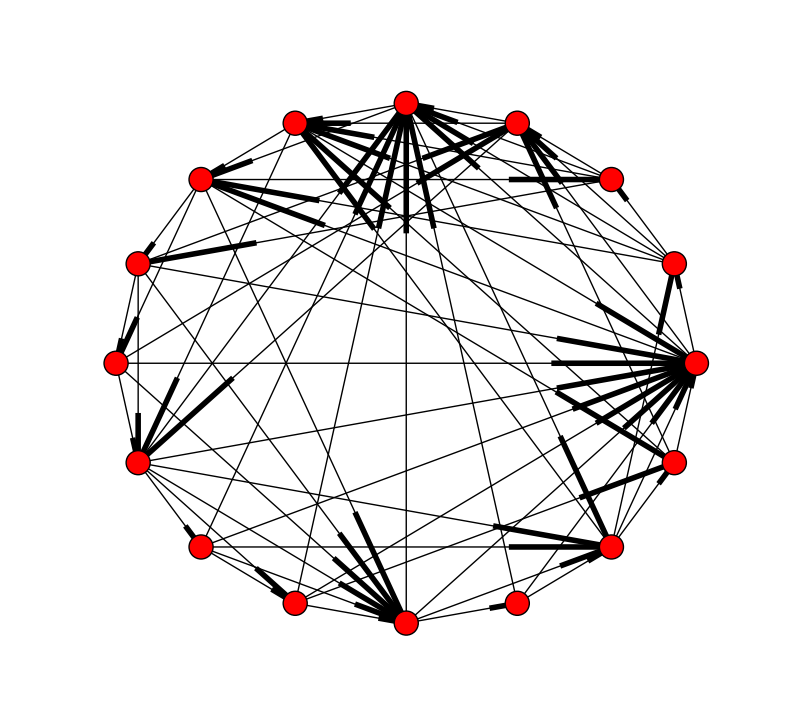
\includegraphics[width=\linewidth]{chordreal}
\caption{An example size 16 network produced by the simulation.  The lines edges are incoming edges.  Note that, unlike in an ideal Chord network, nodes have differing numbers of incoming and outgoing edges.}
\label{chordreal}
\end{figure}



The first step in the simulation was to create a Chord backbone for the network. By default, 1000 nodes were placed in the network. Nodes were given a random id between 0 and $2^{16}-1$;  with $16$ entries in each finger tables, nodes could find any node within $\log_{16}(|network|)$ steps on average.  All traffic travels over the routes created by the Chord protocol. An example of a size 16 network created under the same conditions as our simulated networks can be seen in Figure~\ref{chordreal}.  Once a Chord network was created, IRM was implemented on top that network.   In addition to IRM, we implemented the lazy polling, greedy polling, and poll interception.  Those modifications are collectively referred to as \emph{IRM/LP}.  Both IRM and IRM/LP handle incoming requests during outstanding polls by forwarding those message requests.


\subsection{File Distribution}

Each file would change at a different rate, chosen randomly along a triangular distribution along 0.15 seconds and 100 seconds (we use seconds for simplicity; the actual unit is moot).  A file that changed every 100 seconds was effectively immutable, as the simulation runs for only 100 seconds; this was the same time used in the original IRM simulations \cite{IRM}.    To examine the performance of IRM and IRM/LP in networks with different levels of mutable files, we altered the mean of the triangular distribution.  By default, the file change mean was placed at 100.0 seconds, which resulted in networks with a great number of immutable files.  This setting closely mimics the file change rates used in the simulations in \cite{IRM}.


\subsection{Messages}
Messages were randomly initiated throughout the network.  In real world scenarios, it can be assumed that most of the traffic for a file would originate from only a few locations, enabling the "smarter" creation of replicas. We would be able to assume that nodes that sent a message would be likely to send a similar message in the future. By allowing messages to be sent from random nodes to randomly chosen file owners, we effectively are forcing the file replication protocol to work under a worst-case scenario, where many of the replicas may prove to be utterly useless. 


When a node wants to send a message, it places a message with itself as the source in its inbox.  As the node iterates over its inbox, it tracks the number of messages it is forwarding from other nodes for specific flies.  In addition, when it finds a message with itself as the source, it updates its file query rate for that file.  

Once the forwarding or query rate for that file passes a threshold, it will create a replica for the file. In order to guarantee that we had an adequate number of replicas, we set the query threshold to $0.5 \frac{message}{second}$ and the forward threshold to $1 \frac{message}{second}$.  Once a node creates a replica, it begins polling every 0.15 seconds. If the poll showed the file had yet to change, the amount of time between polls would increase by 0.5 seconds.  If a poll revealed the data was stale, we decreased delay between polls by $66\%$. This puts $\alpha$ and $\beta$ at 0.5 and 1.5, respectively.


Sending a message over an edge creates a slight delay, between 0.05 seconds and 0.1 seconds (note that this substantial portion of the most frequent rate a file can change at).  We assumed that each edge had a 99\% reliability, so the network could expect 1 out of every 100 messages to be dropped.  A dropped message once will effectively take three times longer to arrive at its destination.


Our simulation parameters and their respective results are given in the graphs and discussed below. Note that file requests and polls are kept distinct.




\section{Results}


Our graphs summarize the results of varying the file size of the network and the rate at which files change.  We use three different metrics to measure the effectiveness of our algorithms: the percentage of file requests that result in valid data (the hit rate), the ratio of file requests handled by replicas, and the number of hops that are traveled by poll messages and responses.






\subsection{Effects on Hit Rate}

\begin{figure}
\includegraphics[width=\linewidth]{ratevhitrate}
\caption{IRM/LP and IRM both perform about the same in terms of hit rate, with some deviation.}
\label{ratevhit}
\end{figure}



\begin{figure}
\includegraphics[width=\linewidth]{sizevhitrate}
\caption{IRM/LP and IRM react the same to changes in network size.  The difference in hit rate is due to the difference seen in  Fig.~\ref{sizevload}.}
\label{sizevhit}

\end{figure}



The simulations indicate that IRM/LP is able to handle more frequent file changes better than IRM alone, as shown in Figure~\ref{ratevhit}. % This can be attributed to the poll interception process, which will keep replicas more up-to-date.
However, Figure~\ref{sizevhit} shows IRM having approximately a $1\%$ better hit rate under different network sizes.

The slight reduction in hit rate is to be expected from the increased number of messages that are handled by replicas, as seen in Figures \ref{ratevload} and  \ref{sizevload}.  This is because less messages reach the file owner, who, unlike replicas, will always respond correctly.   In other words, the more work taken off of the file owners, the more chances there are to give stale data back to requesters.

Minor deviations aside, IRM and IRM/LP react the same way to changes in either the size of the network or to file change rates.  Neither set of simulations strongly indicated a substantial loss in hit rate from either algorithm. We can conclude that using IRM/LP will not adversely impact a network's hit rate.

\subsection{Effects on File Request}

\begin{figure}
\includegraphics[width=\linewidth]{ratevload}
\caption{Replicas using IRM/LP handle more file requests for the file owners.}
\label{ratevload}
\end{figure}




\begin{figure}
\includegraphics[width=\linewidth]{sizevload}
\caption{Replicas in IRM/LP performs better at handling requests regardless of the network size.}
\label{sizevload}
\end{figure}





When compared to IRM, our improvements are able to consistently divert substantially more file requests towards replicas, reducing the stress on file owners.  Figure~\ref{ratevload} shows that IRM/LP is responding to 5\% more messages on average than IRM, with the gap in performance growing as files update more often.  

The data presented in Figure~\ref{sizevload} also has IRM/LP outperforming IRM.  In small networks, replicas using  either algorithm respond to a greater number of file requests than in smaller networks, but IRM/LP has an advantage that only grows with the size of the network.

Replicas in both IRM  and IRM/LP will not respond to file requests when it has an outgoing poll.  IRM/LP spends less net time waiting for polls to respond and needs to poll less often, reducing the size of the window in which a replica cannot respond and decrease the frequency at which these events can occur. 


By diverting greater amounts of file requests away from file owners, IRM/LP improves on the goal of creating replicas to handle network traffic.

\subsection{Effects on Polling}

\begin{figure}
\includegraphics[width=\linewidth]{ratevusage}
\caption{IRM/LP consistently reduces the amount of polling traffic under any file change rate.}
\label{ratevusage}
\end{figure}



\begin{figure}
\includegraphics[width=\linewidth]{sizevusage}
\caption{IRM/LP reduces the load on the network induced by polling requests, regardless of the size.}
\label{sizevusage}
\end{figure}

\begin{table}
    \centering
	\begin{tabular}{|r||r|r|r|} \hline 
		Simulation & IRM & IRM/LP & Poll Interceptions \\ \hline \hline
		  10 node network & 566.600& 507.100 &161.200\\ \hline
		 100 node network & 620.333& 595.333 &224.833\\ \hline
		 250 node network & 626.600& 597.333 &203.400\\ \hline
		 500 node network & 581.600& 607.000 &208.200\\ \hline
		1000 node network & 635.333& 586.667 &205.000\\ \hline \hline
		0.15 $sec$ mean change& 727.167& 685.667 &185.000 \\ \hline
		25 $sec$ mean change& 656.000& 645.000&204.333\\ \hline
		50 $sec$ mean change& 657.000& 597.667&201.000\\ \hline
		75 $sec$ mean change& 591.667& 558.000&172.667\\ \hline
		100 $sec$ mean change& 578.667& 557.000&173.667\\ \hline
	\end{tabular}
	\caption{Average number of polls generated for each set of simulations.}
	\label{polltable}
\end{table}


Using IRM/LP we were able to reduce the number of polls by approximately 7\% with IRM/LP, as seen on Table~\ref{polltable}. Besides having less polls overall, we are also seeing fewer network resources being used by the polls.  This can be seen in Figure~\ref{ratevusage}, where the network usage markedly lower for any distribution of file change rates.  The effect is less exaggerated in when the network size is varied, shown in Figure~\ref{sizevusage}, but still indicates noticeable improvement in  almost all cases.



The reduction in network usage is due to multiple attributes.  First, lazy polling causes the delay between polls to grow much slower.  However, this effect is corrected by delaying the polls until the last minute.  

Furthermore, greedy polling also allows poll responses to service multiple replicas, reducing number of polls sent throughout the network.

Poll interception possibly has the greatest impact. On average, replicas handled approximately $33\%$ of the polls.  By allowing replicas along the path to a file owner to answer polls intended for the file owner, the average round trip time for a poll and its response will always be lower.  Polls traveling a shorter distance reduces the overall traffic on the network, as proven previously.


The simulations conclusively show that IRM/LP substantially reduces the overhead created by polls, which is the primary cost of performing consistency maintenance.






\section{Conclusions and Future Work}
In this paper, we considered P2P networks where various nodes make replicas
of files that are frequently requested. The intent of creating replica nodes
is to lessen the burden on the host nodes of the files. The issue that arises is how to ensure that replicated files are up to date without creating so much traffic as to defeat the point of creating replicas in the first place.

Our work is is based on the IRM algorithm, but includes some modifications to improve the performance of the network. Our simulations showed that IRM/LP maintains file consistency at the same level as IRM, but with a decreased level of traffic throughout the network. Replicas send less polls, respond to more messages, and handle polls for file owners, allowing  file owners to avoid becoming overwhelmed by messages. Another benefit to having the replicas handle requests is that the polling and/or file requests do not typically have to travel across as many hops as before, thus reducing the average latency in the network.

There a couple of directions possible for future research. One direction is to further improve the algorithm by finding more ways replicas can handle the load. We can also see if IRM/LP performs any better under different DHT protocols, or if attributes of a particular DHT protocol can be modified or leveraged to reduce the number of stale files in the network. Another direction is using aspects of this algorithm in wireless sensor networks; the file replication aspect of IRM/LP seems to be well suited to the data-centered approach desired in wireless sensor network routing algorithms.  

%In conclusion, we can intelligently create replicas of mutable files while being able to handle the additional overhead created by the polling process.

%Our simulations showed that IRM/LP provides the same level of up-to-date data as IRM, but with a decreased level of traffic throughout the network.  Replicas send less polls, respond to more messages, and handle polls for file owners; this allows file owners to avoid becoming overwhelmed and for messages responses to come back to the their sender much quicker than before.

%There  are a couple of apparent directions for future research. One direction is to directly improve the algorithm, finding more ways replicas can handle the load.  We can also see if IRM/LP performs any better under different DHT protocols, or if attributes of a particular DHT protocol can be modified or leveraged to reduce the number of stale files in the network.


%Another area is using aspects of this algorithm in wireless sensor networks; the file replication aspect of IRM/LP seems to be well suited to the data-centered approach desired in wireless sensor network routing algorithms. 
%THE SIMULATION CODE IS FREELY AVAILABLE WHEN 


%https://github.com/BrendanBenshoof/IRM_LP_SIM

\bibliographystyle{plain}
\bibliography{IRMLP}


\end{document}
